\documentclass[tikz, border=10pt]{standalone}
\usepackage{iftex}
\ifluatex
  \usepackage{fontspec}
  \usepackage{unicode-math}
  \setmainfont{Fira Sans}
  \setmonofont{Fira Mono}
  \setmathfont{Fira Math}
\else
  \usepackage{newpxmath}
\fi

\newcommand{\semihuge}{\fontsize{22}{26}\selectfont}
\usepackage{pgfplots}
\pgfplotsset{compat=1.18}

\begin{document}
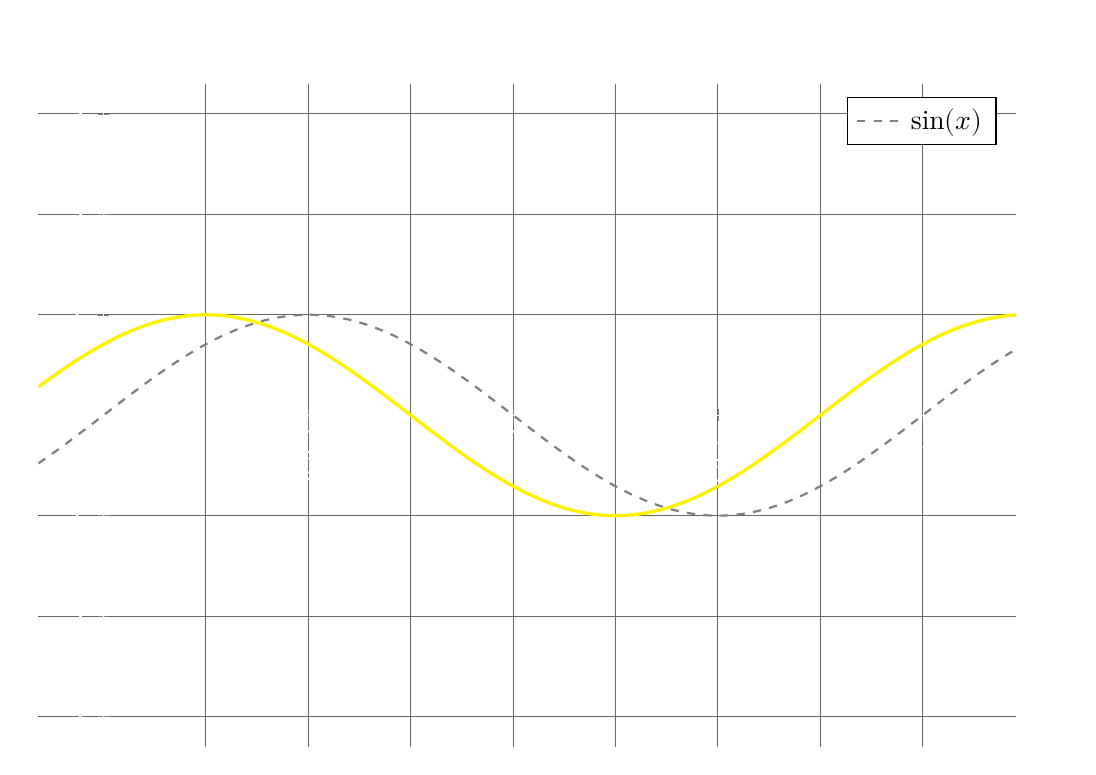
\begin{tikzpicture}
\begin{axis}[
  width=14cm,
  height=10cm,
  xmin=-0.5, xmax=7,
  ymin=-3.3, ymax=3.3,
  % X ticks every pi/4
  xtick={
    0,
    % 0.7854,  % pi/4
    1.5708,  % pi/2
    % 2.3562,  % 3pi/4
    3.1416,  % pi
    % 3.9270,  % 5pi/4
    4.7124,  % 3pi/2
    % 5.4978,  % 7pi/4
    6.2832   % 2pi
  },
  xticklabels={
    $0$,
    % $\frac{\pi}{4}$,
    $\frac{\pi}{2}$,
    % $\frac{3\pi}{4}$,
    $\pi$,
    % $\frac{5\pi}{4}$,
    $\frac{3\pi}{2}$,
    % $\frac{7\pi}{4}$,
    $2\pi$
  },
  xticklabel style={font=\LARGE, white},
  % Y ticks every unit
  ytick={-3,-2,-1,0,1,2,3},
  yticklabel style={font=\Large, white},
  % Extra grid lines at pi/4 positions (no labels)
  extra x ticks={0.7854, 2.3562, 3.9270, 5.4978},
  extra x tick labels={},
  extra x tick style={grid=major, grid style={white!40!black, thin}, tick style={draw=none}},
  % Grid
  grid=major,
  grid style={white!40!black, thin},
  % Axes
  axis lines=center,
  axis line style={-stealth, thin, white},
  xlabel={\huge$x$},
  ylabel={\huge$y$},
  xlabel style={at={(axis cs:7,0)}, anchor=west, white},
  ylabel style={at={(axis cs:0,3.3)}, anchor=south, white},
]
  \addplot[gray, thick, dashed, domain=-0.5:7, samples=200] {sin(deg(x))}; \addlegendentry{$\sin(x)$}
  \addplot[yellow, very thick, domain=-0.5:7, samples=200] {sin(deg(x+pi/4))}; 
\end{axis}
\end{tikzpicture}
\end{document}
